\documentclass[a4paper,conference]{IEEEtran}
\usepackage{latexsym}
\usepackage{amsthm, amsmath, amssymb, amsfonts} % math mode
\usepackage{bm} % bold
\usepackage{cite}
\usepackage[dvipdfmx]{graphicx}
\usepackage{booktabs}
\usepackage{comment}
\usepackage{url}

\begin{document}

\title{Tsallis Entropy Based Labelling}

\author{\IEEEauthorblockN{Kentaro Goto}
\IEEEauthorblockA{Waseda Univ., JP\\
Email: kentaro.goto@asagi.waseda.jp}
\and
\IEEEauthorblockN{Masato Uchida}
\IEEEauthorblockA{Waseda Univ., JP\\
Email: m.uchida@waseda.jp}
}

% 用語集 %
\begin{comment}
    教師あり分類学習 -> supervised classification
\end{comment}

% 形式 %
\begin{comment}
    texソースでは一行につき一文が基本
    まず日本語
    次の行は英語(一部意訳あり,基本的に日本語の一文は英語でも一文)
\end{comment}

\maketitle

\begin{abstract}
%教師あり分類学習においては,学習モデルの設計やパラメータ値の調整とは別に,訓練データの品質が学習の精度に大きく影響する.
In the field of supervised classification, the quality of training data is essential for the accuracy of learning aside from learning algorithm selection or parameter optimisation.
% 訓練データの品質を高めるためには、与えられたインスタンスが所属するクラスに関するアノテータの考えを、ラベルという形でできる限り正確かつ柔軟に反映させる必要がある。
To improve the quality of training data, it is required to reflect annotators idea on to which class any given instance belongs in the form of label, as flexibly and accurately as possible.
% しかし、機械学習における一般的な問題設定では、インスタンスに付与されるラベルは一律に同数に固定されており、アノテータはこの制約のもとでラベル付けすることが暗黙に仮定されている。
However, in conventional problem settings of machine learning, the number of labels per instance is uniformly fixed at a certain value, and it is implicitly assumed that annotators provide labels under such constraint.
% そこで本論文では、与えられたインスタンスが所属するクラスに関する不確からしさに応じて付与するラベルの個数を選択する手法として、Tsallis entropy based labellingを提案した。
Thus in this paper we proposed Tsallis entropy based labelling as a method of flexibly selecting the number of labels for every single given instance depending on the uncertainty about the class that the instance belongs to.
% 提案手法においては、与えられたインスタンスが所属するクラスについてアノテータが感じる不確からしさが、Tsallis entropyとTsallis self-informationによって表現されている。
In the proposed method, annotator's instinctive uncertainty about the class that an instance belongs to is expressed with Tsallis entropy and Tsallis self-information.
% また、典型的に考えられるいくつかのラベル付け手法に帰着する、という整った数理構造を保持している。
Also, the proposed method has a well organised mathematical structure that it includes some of typical annotation models.
% 提案手法の有効性を評価するための数値実験では、インスタンスに付与される平均ラベル数が同じ場合,付与するラベルの個数を固定するアノテーション手法と比較して、提案手法の方がラベルの精度が向上することを示した。
For evaluation of the proposed method, we conducted an experiment to demonstrate that our proposed method outperforms another annotation model where the number of labels per instance is deliberately set at a fixed value for all the instances, in terms of labels accuracy.
\end{abstract}

\IEEEpeerreviewmaketitle

\section{Introduction}
% 教師あり分類学習における「インスタンスに対する正確なラベル付け問題」の重要さとその困難さ(←コストとはいわない)
% インスタンスに付与されるラベルの正確さを確保することは,教師あり分類学習における重要な要件の一つである.
Securing the accuracy of labels attached to instances is one of the important condition for supervised classification. 
% これは,教師あり分類学習により獲得される分類モデルの精度が,インスタンスに付与されるラベルの正確さに強く依存するためである.
This is because of the fact that the learning accuracy of classification models acquired through supervised learning is strongly dependent of the accuracy of the labels attached to instances.
% しかし,インスタンスが所属するクラスがアノテータにとって明らかでない場合,そのインスタンスに付与すべきラベルを正確に選択することは困難である.
However, when the class that an instance belongs to is unclear to an annotator, it is difficult for one to precisely and accurately select the most desirable label.
% Ishida等は,この困難さを軽減するために,インスタンスが「所属する」クラスを表すラベル(ordinary label)ではなく,「所属しない」クラスを表すラベル(complementary label)を付与する場合における教師あり分類学習を定式化した.
To alleviate this difficulty in annotation, Ishida et al. formulated a supervised classification where each label represents the class that an instance does not belong to (complementary label), instead of the usual type of label that indicates the true class. 
% 与えられたインスタンスの所属クラスがアノテータにとって明らかではない場合,そのクラスを特定してordinary labelを付与するよりも,complementary labelを付与する方が容易であると考えることは自然である.
In cases that the true class for a given instance is not obvious to an annotator, it is natural to assume that providing a complementary label is less laborious compared to specifying the true class as an ordinary label.

%単一のcomplementary label/ordinary labelの概念を一般化したcandidate labelの紹介
% インスタンスに対して単一のcomplementary labelを付与することは,それ以外のすべてのラベルをordinary labelの候補にすることと等価である.
Providing a single complementary label for an instance is equivalent to selecting the rest of all the classes as the candidates of an ordinary label.
% Katsura等は,ordinary labelの候補となるラベルをcandidate labelsと呼んだ.
Katsura and Uchida referred to such labels as candidate labels.
% インスタンスに対して単一のordinary labelを付与することは,candidate labelsの個数が1つであることに対応する.
Providing a single ordinary label for an instance corresponds to the situation where the number of candidate labels is one.
% 彼らは,この観点から,単一のordinary/complementary labelがインスタンスに付与された場合の学習を一般化し,複数のcandidate labelsがインスタンスに付与された場合における学習を定式化した.
From this perspective, they generalised the learning framework with single ordinary/complementary label for an instance and formulated a new framework that utilises multiple candidate labels for an instance.

%candidate labelsの個数が予め固定されることの弊害の指摘
% Ishida等,Katsura等の定式化においては,インスタンスに対して付与されるcandidate labelsの個数はすべてのインスタンスに対して共通である.
In the frameworks formulated by Ishida et al and generalised by Katsura and Uchida, the number of labels per instance is fixed and is common for all the instances in a dataset.
% すなわち,これらの定式化においては,「予め指定された同数のラベルをすべてのインスタンスに対して一律に付与しなくてはならない」という制約をアノテータに課すということを暗黙に仮定している.
In other words, it is implicitly assumed that annotators are under a constraint that "they must provide pre-defined number of labels for all the instances" in such frameworks.
% しかし,この制約は,アノテータの能力に相応したラベル付けを困難なものとし,教師あり分類学習における重要な要件であるラベル付けの正確さの成立を妨げる.
However, this constraint hinders annotation commensurate with annotator's ability, and as a consequence it adversely affects an accurate annotation procedure which is crucial in supervised classification.  
% 例えば,与えられたインスタンスの所属クラスがアノテータにとって明らかであるにもかかわらず単一のcomplementary labelを付与しなければならない場合,その制約がアノテータにとっての妨げとなり,正確なラベル付けが期待できない.
e.g. In cases that an annotator has a clear instinct on the true class for a given instance but is required to provide a single complementary label, the constraint is nothing but an interference against the annotator, and we cannot expect accurate annotation.

%本論文の核心となるアイデア(確信度に応じたラベル付けという考え方)の提示
% この問題の原因は,ラベル付けの対象となるインスタンスが所属するクラスについてアノテータが考える不確からしさ,uncertainty(あるいは確からしさ,certainty)はすべてのインスタンスについて均一であるとは限らず,それぞれのインスタンスについてまちまちであることにある.
The cause of this problem is the fact that an annotator's opinion on uncertainty (or certainty) about the class that each instance belongs to is not necessarily uniform for all the instances.
% インスタンスの所属クラスとして不確からしさが低い場合(確からしさが高い場合)には該当するラベルをすべて付与し,そうではない場合にはラベルを付与しない,というように,アノテータの判断によりそれぞれのインスタンスに対してラベル付けするならば,付与するラベルの個数に関する不自然な制約が加えられることはなく,正確なラベル付けを期待できる.→(修正)インスタンスの所属クラスとして不確からしさが低い(確からしさが高い)ものについては、該当するラベルをすべて付与することとすれば、付与するラベルの個数に関する上述したような不自然な制約が加えられることはなく,正確なラベル付けを期待できる.
By allowing annotators to select all the possible candidates as labels as long as their uncertainty (or certainty) about being the true class for a given instance is low (or high) enough, the method is free of the unnatural constraint described above, and we can expect more accurate annotation.
% 本論文では,この着想に基づき,「インスタンスが所属するクラスについてアノテータが考える不確からしさ(確からしさ)が,ある閾値を下回った(上回った)場合に,それに該当するすべてのクラスのラベルを付与する」という原理に基づくラベル付けの振る舞いについて検討し,その特徴を明らかにする.
Based on the idea above, in this paper we investigate behaviours and clarify some important properties of the annotation models whose fundamental structure is "selecting all the possible candidate classes as labels whose uncertainty (or certainty) whether an instance belongs to those are rated higher (or lower) than a threshold".

%数理構造の美しさを強調する
% 本論文では,この不確からしさ(確からしさ)をTsallis self-information,閾値をTsallis entropyにより定量的に表現する枠組みとして,Tsallis entropy based labelling,を提案する.
In this paper, we propose Tsallis entropy based labelling as a framework of expressing the uncertainty by Tsallis self-information and the threshold by Tsallis entropy.
% Tsallis entropyは,Shannon entropyを非加法的に拡張したものである.
Tsallis entropy is a non-additive generalisation of Shannon entropy.
% Tsallis entropyの非加法性はパラメータ$q>0$により制御され,$q\rightarrow 1$の場合がShannon entropyに相当する.
Non additivity of Tsallis entropy is controlled by parameter $q$, and $q \rightarrow 1$ represents Shannon entropy.
% Tsallis entropy based labellingは,インスタンスのラベル付けにおける二つの標準的な手法を特別の場合として含んでいる.
Tsallis entropy based labelling includes two standard labelling methods as its special cases. 
% 一つ目は,インスタンスが所属するクラスについての確率が最も大きいものに対応するラベルを付与するという方法である.
The first one has a structure that it selects the class with highest probability an instance belonging to as a label. 
% この方法は,インスタンスに対して単一のordinary labelを付与する上で自然である.
This concept is natural regarding the purpose of providing a single ordinary label for an instance.
% 本論文では,この方法が,Tsallis entropy based labellingにおいては,$q\rightarrow\infty$の場合に相当することを示す.
In this paper we prove that it is the case of $q \rightarrow \infty$ in the framework of Tsallis entropy based labelling.
% 二つ目は,インスタンスが所属するクラスについての確率が$1/M$を超えるものに対応するすべてのラベルを付与するという方法である.
The second one has a structure that it selects all the classes whose probability of being the true class of an instance is above $1/M$ as labels.
% ここに,$M$は総クラス数を表す.
$M$ indicates the total number of classes.
% この方法は,インスタンスに対して複数のordinary labelを付与する上で自然である.
This concept natural regarding the purpose of providing multiple ordinary labels for an instance.
% 本論文では,この方法が,Tsallis entropy based labellingにおいては,$q\rightarrow 0$の場合に相当することを示す.
In this paper, we prove that it is the case of $q \rightarrow 0$ in the framework of Tsallis entropy based labelling.
% 以上の結果は,Tsallis entropy based labellingが,インスタンスのラベル付けにおける諸手法を一般化したものであることを意味している.
Our theoretical results above point to the fact that Tsallis entropy based labelling is a generalisation of several typical annotation models.

%冒頭の前振りで示したラベル付けの正確さという課題(建前上の目標規定文(より強調したいのは↑の数理構造の美しさ))が解消されたことを示す
% また,本論文では,Tsallis entropy based labellingにより付与されたラベルの正確さを,予め指定された同数のラベルをすべてのインスタンスに対して一律に付与する手法における正確さと比較する.
Also in this paper we compare accuracy of labels generated by Tsallis entropy based labelling and that of those generated by a model that selects a fixed number of labels for all the instances.
% 具体的には,インスタンスが所属するクラスについての確率の上位$k$個に対応するラベルを付与する手法(top-$k$ labelling)との比較を行う.
To be more specific, a comparison method always provides $k$ labels (top-$k$ labelling) corresponding to top $k$ of probabilities of each class being the true class of an instance.
% 数値実験によって,Tsallis entropy based labellingにより付与されたラベルの正確さは,top-$k$ labellingにより付与されたラベルの正確さよりも高いということを示す.
Our numerical experiments demonstrates that the accuracy of the labels generated by Tsallis entropy based labelling is higher than that of those generated by top-$k$ labelling.
% このことは,インスタンスに付与するラベルの個数を同数に固定するという制約を課さずに,アノテータが感じる不確かさに応じて自由に選択させることで,インスタンスに付与されるラベルの正確さが向上することを示唆する.
The result indicates the fact that allowing annotators to freely select arbitrary number of labels for each instance based on their subjective uncertainty (in other words with no constraint of setting a fixed value as the number of labels per instance) enables them to annotate with higher accuracy.

%お約束の論文の構成について
% 本論文の構成は以下の通りである.
This paper is organised as follows.
% 第\ref{sec:related_work}節では、関連研究を概観し、本論文の位置付けを明らかにする。
Section~\ref{sec:related_work} provides an overview of our related works and clarifies the stance of this paper. 
% 第\ref{sec:formulation}節では、Tsallis entropy based labellingを定式化し、その数理構造を明らかにする。
In section~\ref{sec:formulation} we formulate Tsallis entropy based labelling and investigate its mathematical properties.
% 第\ref{sec:numerical_experiment}節では、Tsallis entropy based labellingとtop-$k$ labellingを数値実験により比較し、提案手法の有効性を示す。
Then in section~\ref{sec:numerical_experiment} we compare Tsallis entropy based labelling and top-$k$ labelling in an experiment and demonstrate superiority of our proposed method.
% 第\ref{sec:conclusion}節は、本論文の結論である。
Finally section~\ref{sec:conclusion} concludes this paper.

\section{Related Work}\label{sec:related_work}
% 教師あり分類学習の全体プロセスの出発点は,与えられたインスタンスに対してラベル付けするためのアノテーションを行うことである.
The starting point of the entire processes of supervised classification is the annotation process of providing appropriate labels to given instances. 
% これにより,学習の実行に必要となる訓練データを準備することができる.
This is the preparation step of training data, which is essential for the process of learning.
% 本節では,アノテーションに関する既存手法を概観し,本研究の位置付けを明らかにする.
In this section we take an overview of some existing annotation methods to clarify the stance of this paper.
% \ref{subsec:cost_reduction}節では,大量のインスタンスに対するラベル付けの作業を効率化するための既存手法について紹介する.
Section~\ref{subsec:cost_reduction} lists up existing annotation methods that are specially designed for providing labels to instances in large quantities.  
% \ref{related_comp-labels}節では,インスタンスとそれに対応するラベルの関係が一対一とは限らない場合におけるラベル付けの概念について紹介する.
Section~\ref{related_comp-labels} introduces the annotation concept with no constraint of one label for one instance.
% また,そのようなラベル付けを行うアノテータの振る舞いを規定するモデルについても紹介する.
There are descriptions about some models that are regulated by such annotation behaviours as well.

% \subsection{アノテーションの効率化に関する研究}\label{subsec:cost_reduction}
\subsection{Existing researches about annotation efficiency}\label{subsec:cost_reduction}
% 静止画,動画,3Dモーション,自然言語,ゲノム情報といった様々な応用領域におけるアノテーションの研究が活発に行われている\cite{Zhang:2012,Russakovsky:2015,Muller:2009,Bird:2013,Richardson:2012}.
There are various researches on annotation for data in various application fields, such as image/video recognition, 3D motion capturing, natural language processing, genome information analysis, etc.\cite{Zhang:2012,Russakovsky:2015,Muller:2009,Bird:2013,Richardson:2012}.
% こうした応用領域におけるアノテーションにおいては,高度な専門性に基づいた人間の解釈が求められることがあり, ルールベースの単純な自動アノテーションでは,その精度を十分に確保することが難しい場合がある.
In such application fields, there are cases that high-leveled knowledge or special skills are required for annotation, which makes the task difficult for automatic annotation systems controlled by simple rules, and they may not always achieve enough labels accuracy.
% 一方で,人間による手動アノテーションは一般に高コストなため,アノテーションの手続きの工夫による効率化が必要である.
On the other hand, since manual annotation by human annotators requires high cost in general, some modification has to be taken on annotation procedure.
% そのため,このような具体的な応用領域におけるアノテーションについては,それぞれの応用領域に特有の条件を加味することで,精度と効率を両立するための手法が検討されている.
For the reasons above, in such specific application fields researchers take each field's special properties into consideration when designing annotation procedure to achieve both high accuracy and efficiency.

% また,active learningを用いることで,アノテーションを効率化する手法が提案されている.
Also, there are some methods proposed to achieve higher annotation efficiency in the framework of active learning.
% Active learningは,ラベルが付与されていないインスタンスの中から,分類モデルの性能向上に有効であると期待されるものから順にラベル付けして学習する手法である.
Active learning is a family of learning algorithms that utilises a queue of queries for annotation; the annotator in this framework generates a label for an instance sampled from a group of unlabelled instances in the descending order of their expected effectiveness towards learning model's performance improvement.
% ラベル付けすべきインスタンスを選択する手法は,訓練モデルの性能向上に寄与すると期待される度合いを評価する基準や,適用する機械学習アルゴリズムの違いにより数多く提案されている \cite{Settles:2009,Wang:2011}.
For determination method of which instance to be labelled, there are variety of different ideas proposed depending on what standard to be adapted for assessing the expected effectiveness towards learning model's performance improvement or what learning algorithm to be used~\cite{Settles:2009,Wang:2011}.

% 例えば,Schein等は,ロジスティック回帰にactive learningを適用する手法を提案している\cite{Schein:2007}.
For example, Schein and Ungar proposed a method of applying active learning to Logistic regression~\cite{Schein:2007}.
% また,Fukushi等は,識別境界に近いデータに対してラベルを付けるというactive learningをensemble learningと組み合わせる手法を提案し,それをサイバーセキュリティにおける脅威として知られる悪性ドメイン名の検知に応用している\cite{Fukushi:2019}.
Also, Fukushi et al. proposed a method of applying active learning with annotation procedure of providing labels to instances around the decision boundary, and combining it with ensemble learning to detect malicious domain names which is known as a threat in the field of cyber security~\cite{Fukushi:2019}.

% \subsection{多様なラベル付きデータを用いた学習に関する研究}\label{related_comp-labels} 
\subsection{Researches about learning frameworks with various types of labels}\label{related_comp-labels} 
% インスタンスに付与されるラベルには,その形式の違いによって,いくつかに分類される.
Labels attached to instances are classified into several groups by their format. 
% 図~\ref{fig:rw}に代表的なラベル付けの種類を示す.
Fig~\ref{fig:rw} shows some typical types of label concepts.
% 最も素朴なものは,(a) ordinary labelであり,一つのインスタンスに対し,一つのラベルが付与される.
The most simple one is (a) ordinary label, where each instance is provided with a single label that indicates its true class.
% このようなデータを用いた学習は、supervised learningと呼ばれる。
Learning framework with such labels is referred to as supervised learning.
% また,(b) no labelにおいては,インスタンスはラベルを持たない.
In (b) no label, no instance has any labels.
% このようなデータを用いた学習はunsupervised learningと呼ばれる。
Learning framework that utilises such data is called unsupervised learning.
% (a)と(b)が混在する状態が(c) incomplete labelであり、このようなデータを用いた学習はsemi-supervised learningと呼ばれる。
When (a) and (b) coexists in the same dataset, the learning framework is known as semi-supervised learning. 
% さらに,一つのインスタンスに対してラベルの集合が付与されるものを(d) multi-labelsといい,インスタンスの集合に対して一つのラベルが付与されるものを(e) multi-instancesという.
Moreover, when an instance is provided with a set of labels as shown in (d) it is called multi-labels. On the contrary, when a set of instances is attached to a single label as shown in (e) it is called multi-instances. 
% Multi-labelsは、インスタンスが複数の性質をもつ状態を表す概念である~\cite{Tsoumakas:2009}.
Multi-labels is a concept that represents the state where an instance has multiple properties~\cite{Tsoumakas:2009}.
% Multi-instancesは,ある性質をもつインスタンスの候補が与えられている状態を表す概念である~\cite{Dietterich:1997}.
On the other hanmd, Multi-instances is a concept that represents the state where multiple instances with a certain common property is provided~\cite{Tsoumakas:2009}.

\begin{figure*}[t]
\begin{center}
    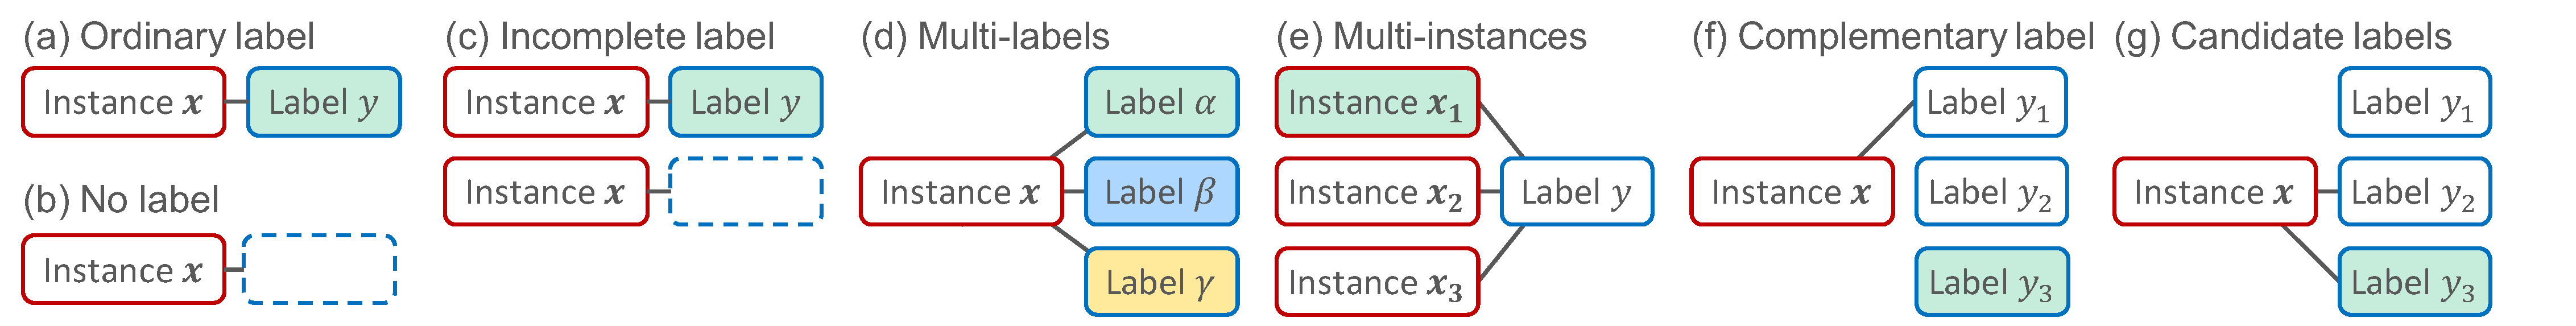
\includegraphics[width=1.0\textwidth]{figs/diagrams/rw_labels.pdf}
    \caption{Six different label types of machine learning frameworks}
    \label{fig:rw}
\end{center}
\end{figure*}

% Ishida等は,インスタンスが所属するクラスがアノテータにとって明らかでない場合に対応するために,インスタンスが所属しないクラスをラベルとするアノテーションを提案している \cite{Ishida:2017}.
Ishida et al. proposed an annotation concept that deals with the cases in which the true class an instance belongs to is not obvious to annotator by making annotators provide a class that an instance \textit{does not} belong to as a label.
% このようなラベルはcomplementary labelと呼ばれる(図~\ref{fig:rw}(f)).
Labels acquired in such annotation are named as complementary label (Fig.~\ref{fig:rw}(f)).
% Ishida等は,complementary labelが付与されたインスタンスを生成する確率分布を,それがordinary labelではない確率によって定義した.
Ishida et al. defined a probability distribution which generates instances assigned to complementary labels as a function of probabilities of each class not being an ordinary label.
% また,Ishida等の結果の一般化に関する研究が行われている.
There are also studies about generalisation of Ishida et al.'s model.
% Katsura等は,インスタンスに対してcomplementary labelsを付与することは,それ以外のすべてのラベルをordinary labelの候補にすることと等価であるということに着目し,ordinary labelの候補となるcandidate labels(図~\ref{fig:rw}(g))が付与されたインスタンスを生成する確率分布を定義した \cite{Katsura:2020}.
Katsura and Uchida focused on the fact that providing a single complementary label for an instance is equivalent to providing the rest of all the classes as the candidates for an ordinary label, and defined a probability distribution that generates instances attached to candidate labels (Fig~\ref{fig:rw}(g)).
% これと等価な確率分布はCao等によっても独立に定義されている \cite{Cao:2020}.
An equivalent probability distribution is also independently defined by Cao and Xu as well~\cite{Cao:2020}.
% また,Feng等は,任意個数のラベルが付与されたインスタンスを生成する確率分布を定義している \cite{Feng:2019}.
Feng and An has defined a probability distribution that generates instances attached to arbitrary number of labels~\cite{Feng:2019}.
% これらの一連の研究により定義された確率分布は,アノテータによるラベル付けの振る舞いを表現するモデルであると捉えることができる.
These probability distributions above can be considered as models that represent annotators' behaviours in labelling procedures.
% しかし,これらの確率モデルにおいては,アノテータが感じる不確かさが与えるインスタンスの精度への影響については議論されていない.
However, in these probabilistic models studies, the effect of the annotators' subjective uncertainty on labels accuracy is never argued.
% 本研究では,「インスタンスの所属クラスについてアノテータが考える不確からしさ(確からしさ)が,ある閾値を下回った(上回った)場合に,そのクラスのラベルを付与する」という原理に基づくラベル付けの振る舞いについて検討し,その特徴を明らかにする.
In our study, we investigate the annotation concept of selecting all the classes as labels whose uncertainty (or certainty) about being the true class of an instance is below (or above) a threshold, and clarify its properties.

\section{Formulation of Tsallis Entropy Based Labelling}\label{sec:formulation}
\subsection{Tsallis Entropy}
% 有限集合$\mathcal{S}$上に定義された至るところ正の確率分布$p$を$p(s) > 0$, $\sum_{s\in\mathcal{S}}p(s)=1$と定義する.
% positive probability distribution $p$ defined on a fine set $\mathcal{S}$ is defined as $p(s) > 0$, $\sum_{s\in\mathcal{S}}p(s)=1$.
% このとき,$\forall q \in \mathfrak{R}_{+}\backslash\{1\}$について,確率分布$p$のTsallis entropy $H_{q}(p)$は以下のように定義される \cite{Tsallis:1988}.
Then $\forall q \in \mathfrak{R}_{+}\backslash\{1\}$, Tsallis entropy $H_{q}(p)$ of the probability distribution $p$ is defined as follows~\cite{Tsallis:1988}.

\begin{align}
    H_{q}(p) = \frac{1}{q-1}\left(1-\sum_{s \in \mathcal{S}}p(s)^{q}\right)\label{eq:tsallis-entropy}
\end{align}
% 式\eqref{eq:tsallis-entropy}において$q \rightarrow 1$とすると,Shannon entropy $H(p)$が得られる.
In Eq.~\eqref{eq:tsallis-entropy}, $q \rightarrow 1$ we have Shannon entropy $H(p)$ as shown below:
\begin{align}
    \lim_{q \rightarrow 1}H_{q}(p) = - \sum_{s \in \mathcal{S}} p(s) \ln p(s) \equiv H(p)\label{eq:shannon-entropy}
\end{align}

% 式\eqref{eq:tsallis-entropy}は,以下のように書き換えることができる.
Eq.~\eqref{eq:tsallis-entropy} can be transformed as

\begin{align}
    H_{q}(p)
    &= \sum_{s \in \mathcal{S}}p(s)\left\{\frac{1}{q-1}(1-p(s)^{q-1})\right\}\nonumber\\
    &=\mathbb{E}_{p}\left[\frac{1}{q-1}\left(1 - p(s)^{q-1}\right)\right]\nonumber\\
    &= \mathbb{E}_{p}[h_{q}(p(s))]
\end{align}
% ここで,$\mathbb{E}_{p}$は$p$に関する期待値を表す.
$\mathbb{E}_{p}$ is the expected value of $p$.
% また、$h_{q}(p(s))$はTsallis self-informationと呼ばれ,以下のように定義される.
$h_{q}(p(s))$ is referred to as Tsallis self-information and is defined as follows:
\begin{align}
    h_{q}(p(s)) = \frac{1}{q-1}\left(1 - p(s)^{q-1}\right)\label{eq:tsallis-self-information}
\end{align}
% すなわち,Tsallis entropy $H_{q}(p)$はTsallis self-information $h_{q}(p(s))$の$p$に関する期待値である。
i.e. Tsallis entropy $H_{q}(p)$ is the expected value of Tsallis self-information about $p$.
% 式\eqref{eq:tsallis-self-information}において$q \rightarrow 1$とすると,Shannon self-information $h(p(s))$が得られる.
In Eq.~\eqref{eq:tsallis-self-information}, $q \rightarrow 1$ gives us Shannon self-information $h(p(s))$, that is, 
\begin{align}
    \lim_{q \rightarrow 1}h_{q}(p(s)) = - \ln p(s) \equiv h(p(s))\label{eq:shannon-self-information}
\end{align}

\subsection{Definition}
% 教師あり分類学習においては,入力$x$と,それが所属するクラスを表すラベル$y \in \mathcal{Y}$を対にした訓練データが必要となる.
For supervised classification, training data is required in the form of a pairs of an input $x$ and a label $y \ in \mathcal{Y}$ that indicates the class that $x$ belongs to.
% $M~(\geq2)$値分類問題においては,$|\mathcal{Y}| = M$となる.
For $M~(\geq2)$-class problem, $|\mathcal{Y}| = M$.
% インスタンス$x$が与えられたとき,その所属クラスが$y$となる条件付き確率を$p_{x}(y)$と表す.
The conditional probability of $y$ being the true class of an instance $x$ is $p_{x}(y)$.
% この条件付き確率分布は,機械学習の文脈においては,真の分布と呼ばれる.
In the context of machine learning, such conditional probability distribution is referred to as "the true distribution".
% アノテータによるラベル付けにより訓練データを生成する場合においては,入力$x$が与えられたとき,それが所属するクラスが$y$であるとアノテータが考える条件付き確率が$p_{x}(y)$に対応する.
In cases human annotators generate labels for training data, the conditional probability of $y$ being the true class of an instance $x$ that annotators instinctively assess corresponds to $p_{x}(y)$.

% 図~\ref{fig:rw}(a)のordinary labelにおいては,条件付き確率$p_{x}(y)$に従って選択された一つのラベルが入力$x$に対して付与されることが仮定されている.
In the framework of Fig.~\ref{fig:rw}(a) ordinary label, it is assumed that one label $y$ that is generated from the conditional probability $p_{x}(y)$ is assigned to an instance $x$.
% インスタンス$x$が所属するクラスについてアノテータが感じる不確からしさがこの条件付き確率$p_{x}(y)$により定まるものとし,それを$f(p_{x}(y))$と表す.
Annotator's subjective uncertainty about the true class of an instance $x$ is regulated by the conditional probability $p_{x}(y)$, and is denoted as $f(p_{x}(y))$.
% 本論文では,この不確からしさ$f(p_{x}(y))$が,ある閾値を下回った場合にそのクラスのラベルを付与する,という原理に基づくラベル付けの振る舞いについて調べる.
In this paper we investigate the behaviours of the annotation model based on the principle of providing all the classes as labels whose uncertainty $f(p_{x}(y))$ is below a threshold.
% また,この閾値は,条件付き確率分布$p_{x}$の汎関数$\theta(p_{x})$として定まるものとする.
The threshold mentioned above is determined by a functional $\theta(p_{x})$ of the conditional probability distribution $p_{x}$.
% 具体的には,この閾値$\theta(p_{x})$を,$f(p_{x}(y))$の$p_{x}(y)$に関する期待値として以下のように定義する.
To be more specific, we define the threshold $\theta(p_{x})$ as the expected value of $f(p_{x}(y))$ about $p_{x}(y)$. 
\begin{align}
    \theta(p_{x})
    = \mathbb{E}_{p_{x}}[f(p_{x}(y))]
    = \sum_{y \in \mathcal{Y}}p_{x}(y)f(p_{x}(y))
\end{align}
% この原理においては,入力$x$に対し,$f(p_{x}(y)) \le \theta(p_{x})$を満たすすべての$y \in \mathcal{Y}$がラベルとして付与される.
In this principle, for any input $x$, any $y \in \mathcal{Y}$ that satisfies $f(p_{x}(y)) \le \theta(p_{x})$ is instantly selected as one of labels.
% 条件付き確率分布$p_{x}$は$x$の関数であることから、閾値$\theta(p_{x})$も$x$の関数となる。
Since the conditional probability distribution $p_{x}$ is a function of $x$, the threshold $\theta(p_{x})$ is also a function of $x$.
% したがって,付与されるラベルの個数は、すべてのインスタンスに対して一律に同数とはならず、インスタンスごとに変化する。
Thus the number of labels for an instance are not necessarily the same and it varies among all the instances.

% ここで,$f(\cdot)=h_{q}(\cdot)$とすると,不確からしさ$f(p_{x}(y))$は$p_{x}(y)$に関するTsallis self-informationに対応し,閾値$\theta(p_{x})$はTallis entropyに対応する.
Here let $f(\cdot)=h_{q}(\cdot)$, then the uncertainty $f(p_{x}(y))$ can be expressed by Tsallis self-information about $p_{x}(y)$, and the threshold $\theta(p_{x})$ by Tsallis entropy.
% このラベル付けの方法を,本論文では,Tsallis entropy based labellingと呼ぶ.
In this paper we call the annotation method described above Tsasllis entropy based labelling.
% この方法においては、与えられたインスタンス$x$の所属クラスが$y$であるということについての不確からしさ$h_{q}(p_{x}(y))$が、インスタンス$x$の所属クラスについての不確からしさの期待値である$H_{q}(p_{x})$を下回った場合に、インスタンス$x$に対してラベル$y$が付与される。
In this model, label $y$ is assigned to an instance $x$ when the uncertainty whether the true class of the instance $x$ is $y$ is lower than the general uncertainty of the true class for the same instance $x$.  
% $h_{q}(p_{x}(y))$と$H_{q}(p_{x})$がいずれも$x$の関数であることから、インスタンス$x$に付与されるラベルの個数は、インスタンスごとに変化する。
Since both $h_{q}(p_{x}(y))$ and $H_{q}(p_{x})$ are function of $x$, the number of labels provided to an instance $x$ differs among each instances.

\subsection{Examples}\label{subsec:example_models}
% Tsallis entropy based labellingの定義に用いられる$h_{q}(p_{x}(y))$と$H_{q}(p_{x})$は、いずれもパラメータ$q$をもつ。
$h_{q}(p_{x}(y))$ and $H_{q}(p_{x})$ that appear in the definition of Tsallis entropy based labelling both have a parameter $q$ in its formulation.
% 以下では、このパラメータ$q$の値を変化させることで、典型的に考えられるいくつかのラベル付け手法が特別な場合として導かれることを示す。
The proof of the fact that some of the typical annotation methods are derived from the proposed method by manipulating the parameter $q$ is described below.
% これらの例より、入力$x$が与えられたとき,それが所属するクラスが$y$であるとアノテータが判断する条件付き確率が$p_{x}(y)$が同一であったとしても、実際にラベル付けを行うかどうかは、パラメータ$q$によって変化することがわかる。
These examples reveal that parameter $q$ is responsible whether an annotator actually selects any designated class $y$, even in the cases where the conditional probability value $p_{x}(y)$ is exactly the same for multiple different $y$s.
% すなわち、このパラメータ$q$は、アノテータがラベル付けを行う際のポリシーの違いを表すものと解釈することができる。
In other words, the parameter $q$ can be interpreted as a measurement of difference in each annotator's labelling policies.

% \subsubsection{$q \rightarrow 0$の場合}
\subsubsection{Case 1. $q \rightarrow 0$}
From Eq.~\eqref{eq:tsallis-entropy} and~\eqref{eq:tsallis-self-information}, we have
\begin{align}
    f(p_{x}(y)) &= \frac{1-p_{x}(y)}{p_{x}(y)}\label{eq:uncertainty-q=0}\\
    \theta(p_{x}) &= M -1\label{eq:threshold-q=0}
\end{align}
% 式\eqref{eq:uncertainty-q=0}より,$x$の所属するクラスが$y$であることについての不確からしさ$f(p_{x}(y))$が,$x$の所属するクラスが$y$である確率$p_{x}(y)$と,そうではない確率$1-p_{x}(y)$の比によって定められることがわかる.
From Eq.~\eqref{eq:threshold-q=0} it can be stated that the uncertainty about $y$ being the true class for $x$ ($f(p_{x}(y))$) is determined by the ratio of the probability of $y$ being the true class of $x$ ($p_{x}(y)$) to the probability for its complementary event ($1-p_{x}(y)$).
% また,\eqref{eq:threshold-q=0}は,閾値がクラスの総数に依存することがわかる.
Also,~\eqref{eq:threshold-q=0} shows that its threshold is governed by the total number of classes. 
% このとき,
Below is true for such model.
\begin{align}
    f(p_{x}(y)) \le \theta(p_{x}) \Leftrightarrow p_{x}(y) \ge \frac{1}{M}\label{eq:rule-q=0}
\end{align}
% 式\eqref{eq:rule-q=0}より,Tsallis entropy based labellingには,$x$の所属するクラスが$y$である確率$p_{x}(y)$が,$x$の所属するクラスを無作為に選ぶ場合の確率よりも大きい場合にラベル$y$を付与する,という手法が特別な場合として含まれることがわかる.
Eq.~\eqref{eq:rule-q=0} shows that Tsallis entropy based labelling includes a certain model as one of the special cases; a model that assigns all the candidates $y \in \mathcal{Y}$ as labels whose probability of being the true class of $x$ ($p_{x}(y)$) is higher than that for randomly selecting one label.
% 本論文においては,この手法を$1/M$ labellingと呼ぶ.
In this paper we call this annotation method $1/M$ labelling.

% \subsubsection{$q \rightarrow 1$の場合}
\subsubsection{Case 2. $q \rightarrow 1$}
% 式\eqref{eq:tsallis-entropy}, ~\eqref{eq:tsallis-self-information}より.
From~\eqref{eq:tsallis-entropy} and ~\eqref{eq:tsallis-self-information} we have
\begin{align}
    f(p_{x}(y)) &= h(p_{x}(y)) = - \ln p_{x}(y)\label{eq:uncertainty-q=1}\\
    \theta(p_{x}) &= H(p_{x}) = - \sum_{y \in \mathcal{Y}} p_{x}(y) \ln p_{x}(y)\label{eq:threshold-q=1}
\end{align}
% となる.
% 式\eqref{eq:uncertainty-q=0}より,$x$の所属するクラスが$y$であることについての不確からしさ$f(p_{x}(y))$が,$x$の所属するクラスが$y$である確率$p_{x}(y)$のShannon self-informationによって定められることがわかる.
From Eq.~\eqref{eq:uncertainty-q=1} it can be stated that the uncertainty about $y$ being the true class for $x$ ($f(p_{x}(y))$) is determined by Shannon self-information of $p_{x}(y)$, the probability of $y$ being the true class for $x$.
% また,\eqref{eq:threshold-q=0}は,閾値が$p_{x}(\cdot)$のShanonn entropyによって定められることがわかる.
Also,~\eqref{eq:threshold-q=1} shows that its threshold is governed by Shannon entropy of $p_{x}(\cdot)$. 
% このとき,
Below is true for such model.
\begin{align}
    f(p_{x}(y)) \le \theta(p_{x}) \Leftrightarrow p_{x}(y) \ge \exp(-H(p_{x}))\label{eq:rule-q=1}
\end{align}
% が成り立つ.
% 一般に,$H(p_{x}) \le \ln M$であることから,$\exp(-H(p_{x})) \ge 1/M$となる.
Given the fact that $H(p_{x}) \le \ln M$ in general, $\exp(-H(p_{x})) \ge 1/M$ is true.
% したがって,式\eqref{eq:rule-q=1}の手法により入力$x$に付与されるラベルの個数は,式\eqref{eq:rule-q=0}の手法よりも少なくなる.
Therefore the number of labels generated by the method controlled by Eq.~\eqref{eq:rule-q=1} is less than that of Eq.~\eqref{eq:rule-q=0}.
% 本論文においては,この手法をShanonn entropy-based labellingと呼ぶ.
In this paper we call this annotation method Shannon entropy based labelling.

% \subsubsection{$q \rightarrow \infty$の場合}
\subsubsection{Case 3. $q \rightarrow \infty$}
% 以下が成り立つ.
Below is obtained by $q \rightarrow \infty$.
\begin{align}
    &\lim_{q \rightarrow \infty} \frac{\frac{1}{q-1}-H_{q}(p_{x})}{\frac{1}{q-1}-h_{q}(p_{x}(y))}\nonumber\\
    &=\lim_{q \rightarrow \infty} \sum_{z \in \mathcal{Y}} p_{x}(z) \left(\frac{p_{x}(z)}{p_{x}(y)}\right)^{q-1}\nonumber\\
    &
    \begin{cases}
    \le 1, & \text{if~}p_{x}(y) = \max_{z\in\mathcal{Y}}p_{x}(z)\\
    = \infty, & \text{otherwise}
    \end{cases}
\end{align}

% よって,
The equation above can further be rearranged to obtain: 
\begin{align}
    f(p_{x}(y)) \le \theta(p_{x}) \Leftrightarrow p_{x}(y) = \max_{z \in \mathcal{Y}}p_{x}(z)\label{eq:rule-q=infty}
\end{align}
% が成り立つ.
% 式\eqref{eq:rule-q=infty}より,Tsallis entropy based labellingには,$x$の所属するクラスが$y$である確率が最も大きいときに,それに対応するラベルを付与する,という手法が特別な場合として含まれることがわかる.
Eq.~\eqref{eq:rule-q=infty} shows that Tsallis entropy based labelling includes another certain model as one of the special cases; a model that assigns one and only class $y \in \mathcal{Y}$ as a label whose probability of being the true class of $x$ ($p_{x}(y)$) is the maximum in the distribution.
% 本論文においては,この手法をtop-$1$ labellingと呼ぶ.
In this paper we call this annotation method top-$1$ labelling.

\section{Numerical Experiment}\label{sec:numerical_experiment}
% 本節では、Tsallis entropy based labellingを用いたラベル付けの正確さを評価するために数値実験を行う。
In this section we conduct a numerical experiment to evaluate the accuracy of labels generated by Tsallis entropy based labelling.
% 本実験は,アノテータにラベルづけをさせるプロセス,そして得られたラベルの正確さを評価する指標を計算するプロセスの2つで構成される.
This experiment is comprised of two processes; a process of having an annotator to provide labels and a following process of calculating the evaluation measures for labels quality.
% 以下では,まず、これらのプロセスを実行する手順、評価指標、使用するデータセットについて述べる。
We summarise the flow of the processes, evaluation measurements and dataset in the following sections.
% その上で、実験の結果を示し、Tsallis entropy based labellingの有効性を明らかにする。
Then we provide the experiment results to demonstrate the effectiveness of Tsallis entropy based labelling.

\subsection{Experimental Settings}
% \subsubsection{アノテータのモデル化}\label{subsec:annotation_process}
\subsubsection{Modelling an annotator}\label{subsec:annotation_process}
% Tsallis entropy based labellingの定義においては、与えられたインスタンス$x$に対し、その所属クラスが$y$であるとアノテータが判断する条件付き確率分布$p_{x}(\cdot)$が用いられている.
In the formulation of Tsallis entropy based labelling, annotator's conditional probability distribution of $y$ being the true class for an instance $x$ ($p_{x}(\cdot)$) is present.
% この条件付確率分布$p_{x}(\cdot)$は、アノテータの能力や知識、あるいは感覚によって、アノテータが意識することなく決定されるものである。
The conditional probability distribution $p_{x}(\cdot)$ is unconsciously determined by annotator's ability, knowledge or sense (something not rational).
% Tsallis entropy based labellingを用いたラベル付けの正確さを評価するためには、この条件付確率分布$p_{x}(\cdot)$を何らかの方法でモデル化する必要がある。
In order to fully evaluate annotation quality, there is a need of modelling such conditional probability distribution $p_{x}(\cdot)$.
% しかし、この条件付確率分布$p_{x}(\cdot)$を正確にモデル化することは本実験の目的の範囲を超えている。
However, accurate modelling of the conditional probability distribution $p_{x}(\cdot)$ excesses the scope of the purpose of our experiment.
% 本実験の目的は、Tsallis entropy based labellingを特徴づけるパラメータ$q$の値が変化することで、ラベル付けの特性がどのように変化するかを調べることである。
The actual purpose of our experiment is investigation of how properties of annotation changes by manipulating the value of $q$.
% そこで本実験では、適当な機械学習アルゴリズムを用いて識別器を学習し、それをアノテータとみなす。
Thus in our experiment we choose a suitable machine learning algorithm to train a classifier, and use it as an annotator.
% そして、この学習された識別器(アノテータ)に対してインスタンス$x$を入力したときに、その所属クラスが$y$と判断される条件付き確率を$p_{x}(y)$とみなす。
We regard the conditional probability of $y$ being the true class of an instance $x$ that is provided to a pre-trained classifier (annotator) as $p_{x}(y)$.
% アノテータは、条件付き確率分布$p_{x}(\cdot)$を用いたTsallis entropy based labellingによって、与えられたインスタンスに対してラベル付けを行う。
The annotator generates labels to given instances by Tsallis entropy based labelling which is regulated by the conditional probability distribution $p_{x}(\cdot)$.

% \subsubsection{評価指標}\label{subsec:labels_evaluation}
\subsubsection{Labels evaluation measurements}\label{subsec:labels_evaluation}
%前節の方法でラベル付けされた結果を評価する指標について述べる。
% ラベル付けの対象となるインスタンスの集合を$\mathcal{X}$とおく。
Let $\mathcal{X}$ be the set of the instances to be labelled.
% また、インスタンス$x \in \mathcal{X}$に対して付与されたラベルの集合を$\mathcal{Y}_{x} \subset \mathcal{Y}$とおく。
Similarly, let $\mathcal{Y}_{x} \subset \mathcal{Y}$ be the set of labels generated for instances $x \in \mathcal{X}$.
% このとき、平均ラベル数は以下のように定義できる。
The average number of labels is defined as below:
\begin{align}
    \frac{1}{|\mathcal{X}|}\sum_{x \in \mathcal{X}} |\mathcal{Y}_{x}|
\end{align}
% また、付与されたラベルの正確さを評価する指標を以下のように定義する。
To assess the accuracy of generated labels, equation described below is used:
\begin{align}
    \frac{1}{|\mathcal{X}|}\sum_{x \in \mathcal{X}} \frac{1}{|\mathcal{Y}_{x}|} \sum_{y \in \mathcal{Y}_{x}} I(y = y^{*}_{x})
\end{align}
% ここで、$y^{*}_{x} \in \mathcal{Y}$は、インスタンス$x$が所属するの真のクラスを表す。
$y^{*}_{x} \in \mathcal{Y}$ represents the true class of an instance $x$.
% また、$I(\cdot)$は、括弧内が真のときに$1$、偽のときに$0$となるインジケータ関数である。
$I(\cdot)$ is an indicator function that takes the value $1$ when the variable in the parenthesis is true, and takes the value $0$ otherwise.

% \subsubsection{比較手法}\label{subsec:experiment}
\subsubsection{Comparison method}\label{subsec:experiment}
% Tsallis entropy based labellingにおいては、インスタンスが所属するクラスについてアノテータが感じる不確からしさに基づきラベルが付与されるため、付与されるラベルの個数はインスタンスごとに異なる。
In Tsallis entropy based labelling the number of labels per instance varies among instances because labels are generated by evaluating an annotator's uncertainty about the true class for each instance as standard.
% すなわち、不確からしさが高い場合には付与するラベルの個数が増加し、不確からしさが低い場合には付与するラベルの個数が減少する。
That is, more labels are generated for high uncertainty instances, and the opposite for low uncertainty instances.
% 本論文では、このように付与されるラベルの個数を動的に変化させることの有効性を示すために、付与されるラベルの個数を固定した場合との比較を行う。
In this paper we compare the annotation method with dynamically set number of labels to another method with statically set number of labels.

% ラベルの個数を固定する手法として最も自然なものの一つは、インスタンス$x \in \mathcal{X}$について、条件付き確率$p_{x}(y)$が大きいものから順に$k \le M$個のラベルを付与する手法である。
The most simple annotation method with the fixed number of labels is the one that selects the top $k$ of the conditional probabilities $p_{x}(y)$ and providing the corresponding $k \le M$ classes as labels.
% この手法をTop-$k$ labellingと呼ぶ。
We name this method Top-$k$ labelling.
% 本論文では、Top-$k$ labellingとTop-$(k+1)$ labellingを以下のように混合した手法を、Tsallis entropy based labellingと比較する。
In this paper we compare the method of combining Top-$k$ labelling and Top-$(k + 1)$ labelling with Tsallis entropy based labelling.

% まず、$\mathcal{X} = \mathcal{X}_{k} \cup \mathcal{X}_{k+1}$, $\mathcal{X}_{k} \cap \mathcal{X}_{k+1} = \empty$を満たす$\mathcal{X}_{k}$と$\mathcal{X}_{k+1}$を無作為に選択する。
First, we randomly sample $\mathcal{X}_{k}$ and $\mathcal{X}_{k+1}$ that satisfy $\mathcal{X} = \mathcal{X}_{k} \cup \mathcal{X}_{k+1}$, $\mathcal{X}_{k} \cap \mathcal{X}_{k+1} = \empty$.
% そして、$\mathcal{X}_{k}$に含まれるインスタンスについてはTop-$k$ labellingを施し、$\mathcal{X}_{k+1}$に含まれるインスタンスについてはTop-$(k+1)$ labellingを施す。
Next, we apply Top-$k$ labelling to the instances in $\mathcal{X}_{k}$ and also apply Top-$(k+1)$ labelling to the instances in $\mathcal{X}_{k+1}$.
% このとき、平均ラベル数は以下のようになる。
The average number of labels is calculated as below:
\begin{align}
    \frac{k|\mathcal{X}_{k}| + (k+1)|\mathcal{X}_{k+1}|}{|\mathcal{X}|}
\end{align}
% $\mathcal{X}_{k}$に含まれるインスタンスの個数と、$\mathcal{X}_{k+1}$に含まれるインスタンスの個数の比率を変化させることで、平均ラベル数は$k$から$k+1$の範囲を変化する。
By changing the ratio between the number of the instances in $\mathcal{X}_{k}$ and that of $\mathcal{X}_{k+1}$, the average number of labels ranges from $k$ to $k + 1$.
% 本論文では、この一般化された手法を含め、単にTop-$k$ labellingと呼ぶ。
In this paper we simply refer to this generalised method as top-$k$ labelling as well.

% \subsubsection{データセット}\label{subsec:dataset}
\subsubsection{Dataset}\label{subsec:dataset}
% 本実験では,手書き数字の画像データセットであるMNISTを使用する.
In our experiment we use MNIST which is a basic dataset of hand written digits images recognition.
% MNISTには訓練データとして$50000$件,テストデータとして$10000$件が用意されている.
MNIST contains $50,000$ training data and $10,000$ test data.
% MNISTは本来$10$クラス分類を想定したデータセットである。
MNIST is originally designed as a 10-class classification dataset.
% しかし、本論文では、クラス数によるアノテーションの振る舞いの変化を観察するため,10クラスの中から任意の$k$クラス ($2 \le k \le 9$)クラスを選択し、選択された$k$クラスの分類を行う。
However, in order to observe the change in behaviours of annotation methods, we test with all the possible combinations of $k$ classes ($2 \le k \le 9$).
% $k$クラスの選び方については$\binom{10}{k}$通りの組合せがあるが,本研究ではそれらすべての組合せについて実験を行い,それらの平均をとった.
There are total of $\binom{10}{k}$ ways of choosing $k$ classes, so in our study we conducted the same experiment for all the combinations and calculate the average of each results.

% \ref{subsec:annotation_process}節で説明したアノテータを作成するための学習においては,任意のクラスの組合せに対して,訓練データのうち選ばれた組合せのクラスのデータのみを計$2000$件用いる.
For the learning process described in section~\ref{subsec:annotation_process}, $2,000$ training data of only the chosen combination of the classes are used.
% e.g. $2$クラス問題の計算の際,選ばれた組み合わせがクラス$0$とクラス$1$であったなら,訓練データからクラス$0$とクラス$1$に属するものだけを選び出し,そこから$2000$件をアノテータ作成に使用する.
e.g. For binary classification, when class $0$ and class $1$ are chosen, we sample $2,000$ data of class $0$ and class $1$ only as training data for creating the annotator.
% $2000$という数字は$10$クラス問題においてアノテータの精度(accuracy)がおよそ$8$割になるように設定したことに由来する.
The value $2,000$ originates as the number of training data for a classifier to stably achieve around $80 [\%]$ of accuracy.
% この理由は,あまりに精度の低すぎる学習器では人間を模したアノテータとして不適当だと考え,おおよそ$8$割正解できるように調整したことによる.
The reason for this is because we thought that it is not suitable for a classifier that models a human annotator to have too low accuracy.
% 一方で,アノテータに新たにラベルを付与させるインスタンス数も,各$M$クラス問題に対して計$2000$件で固定した.
On the other hand the number of instances to be labelled by the annotator is also fixed at $2,000$.
% すなわち、$|\mathcal{X}|=2000$である。
That is, $|\mathcal{X}|=2000$.

% \subsubsection{実装}\label{subsec:implementation}
\subsubsection{Implementation}\label{subsec:implementation}
% 本研究における実験の実装は全てPythonで行い,機械学習のライブラリにはscikit-learnを使用した.
All the experiments in this study are implemented by Python, and we used scikit-learn for machine learning library.
% なお,~\ref{subsec:annotation_process}節で説明したアノテータをモデル化した学習器としては、多クラス分類のLogistic Regressionを選択した.
Note that for a classifier that models an annotator described in section~\ref{subsec:annotation_process} we selected multi-class Logistic regression. 
% アノテータのモデルの精度を高めることは本研究においては本質的ではないため,特別な特徴量設計やハイパーパラメータの調整は行っていない.
Training an annotator with higher accuracy is not the essential problem in our study, and therefore we have not conducted any special feature-engineering and hyper-parameter optimisation.

\subsection{Experimental Results}
% \subsubsection{パラメータ値による性能変化}\label{subsec:preliminary_exp}
\subsubsection{The performance change by parameter manipulation}\label{subsec:preliminary_exp}
% まず、MNISTに対するTsallis entropy based labellingとTop-$k$ labellingの挙動を確認する.
First we confirm general behaviours of Tsallis entropy based labelling and Top-$k$ labelling against MNIST.
% Tsallis labellingでは,$q\in\{0, 0.1, 0.5, 1.0, 2.0, 10.0, \infty\}$で変動させる.
For Tsallis entropy based labelling $q$ ranges as $q\in\{0, 0.1, 0.5, 1.0, 2.0, 10.0, \infty\}$.
% ただし,$q = 0$と$q = 1.0$と$q = \infty$の場合は、それぞれ$1/M$ labelling($M$は総クラス数),Shannon labelling,Top-$1$ labellingに対応する(第\ref{subsec:example_models}節参照)。
Here $q = 0$, $q = 1$, $q = \infty$ corresponds to $1/M$ labelling, Shannon labelling, Top-$1$ labelling respectively.
% Top-$k$ labellingでは、$k\in\{1, 2, ..., 9\}$で変動させる.
For Top-$k$ labelling the value of $k$ ranges as $k\in\{1, 2, ..., 9\}$.
% 以上の設定のもと、$q$を変化させたときのTsallis entropy based labellingと,$k$を変化させたときのTop-$k$ labellingによるアノテーションを実験で再現し,それぞれに対するラベル精度と平均ラベル数を計算した.
Under the settings described above, we replicated annotation by Tsallis entropy based labelling and Top-$k$ labelling by experiment and calculated labels accuracy and the average number of labels per instance.
 
% まず、Tsallis entropy based labellingについての結果を示す。
First we show the results for Tsallis entropy based labelling.
% 図~\ref{fig:tsallis_acc}は、クラス数とラベル精度の関係を表したグラフである.
Fig.~\ref{fig:tsallis_acc} is a graph that represents the relationship between the number of classes and labels accuracy.
% 横軸がクラス数を,縦軸がラベル精度を表す.
The horizontal axis represents the number of classes, and the vertical axis represents labels accuracy.
% 図~\ref{fig:tsallis_ave_lnum}は、クラス数と平均ラベル数の関係を表したグラフである.
Fig.~\ref{fig:tsallis_ave_lnum} is a graph that represents the relationship between the number of classes and the average number of labels.
% 横軸がクラス数を,縦軸が平均ラベル数を表す.
The horizontal axis represents the number of classes, and the vertical axis represents the average number of labels.
% 図~\ref{fig:tsallis_acc}より,パラメータ$q$を大きくするほどラベル精度が向上する様子を確認できる.
From Fig.~\ref{fig:tsallis_acc} we can observe that larger value for $q$ achieves higher labels accuracy.
% 図~\ref{fig:tsallis_ave_lnum}より,$q$を大きくするほど平均ラベル数は減少し,$1.00$に近づく様子を確認できる.
From Fig.~\ref{fig:tsallis_ave_lnum} we can observe that larger value for $q$ generates less average number of labels, which approaches $1.00$.
% このことから,パラメータ$q$は,アノテータがラベル付けを行う際の積極度を表すことがわかる.
These facts indicate that the parameter $q$ represents assertiveness of an annotator for labelling.

\begin{figure}[t]
\begin{center}
    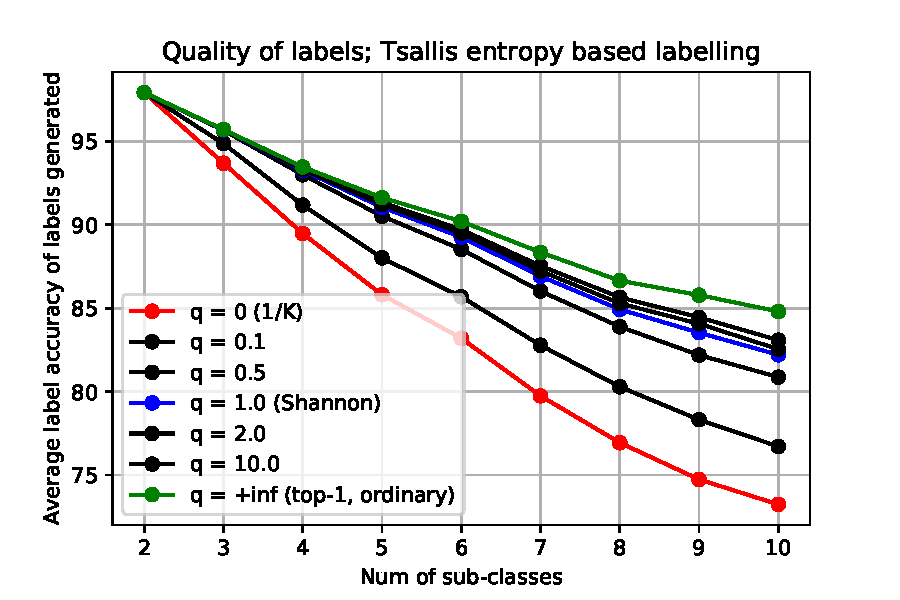
\includegraphics[width=1.0\linewidth]{figs/graphs/tsallis-qs.pdf}
    \caption{Tsallis entropy based labelling - accuracy curve}
    \label{fig:tsallis_acc}
\end{center}
\end{figure}

\begin{figure}[t]
\begin{center}
    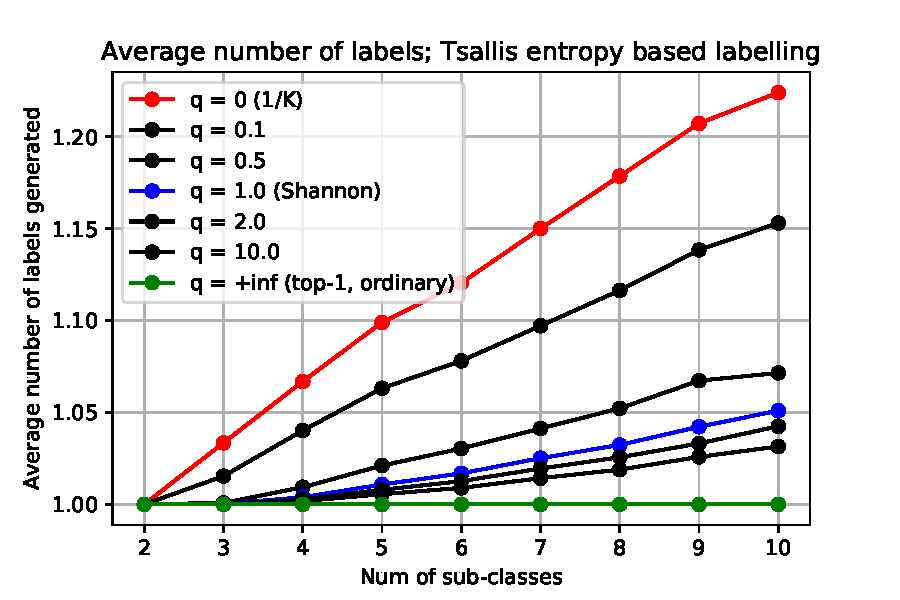
\includegraphics[width=1.0\linewidth]{figs/graphs/tsallis-qs-lnum.pdf}
    \caption{Tsallis entropy based labelling - average number of labels per data}
    \label{fig:tsallis_ave_lnum}
\end{center}
\end{figure}

% 次に,Top-$k$ labellingについての結果を示す。
Next we show the results for Top-$k$ labelling.
% 図~\ref{fig:top-k}はクラス数のラベル精度の関係を表したグラフである.
Fig.~\ref{fig:top-k} is a graph that shows the relationship between the number of classes and labels accuracy.

\begin{figure}[t]
\begin{center}
    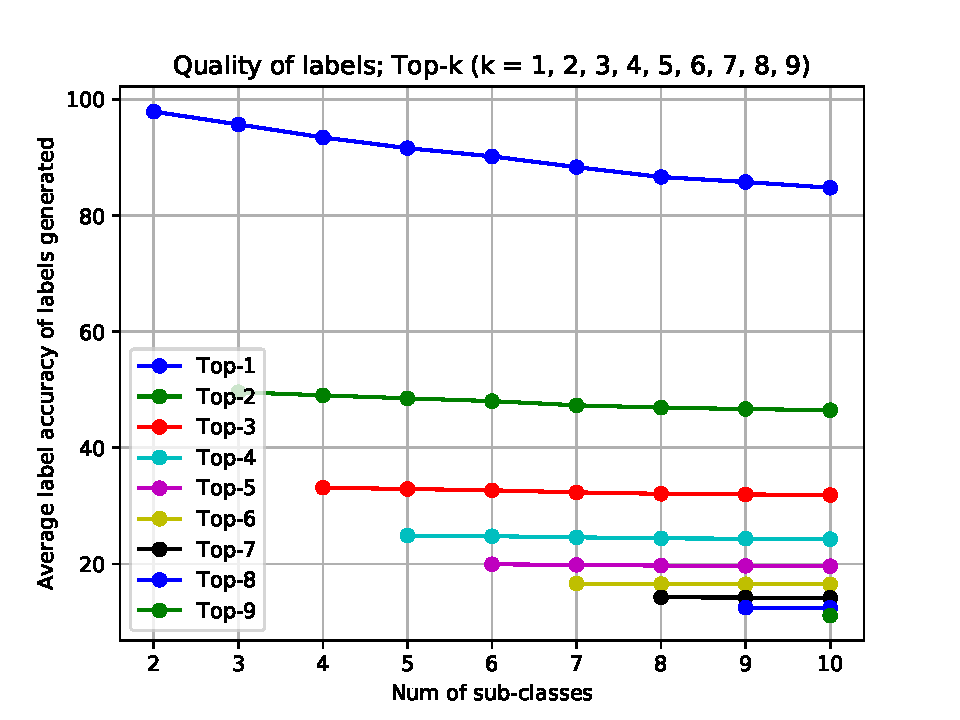
\includegraphics[width=1.0\linewidth]{figs/graphs/topk-labels-acc.pdf}
    \caption{Top-$k$ labelling - accuracy curve}
    \label{fig:top-k}
\end{center}
\end{figure}
% 本図より、$k$の変化に対する精度の変化は,$k$の値が小さいときほど大きいことがわかる.
By observing the figure it can be stated that the change of labels accuracy is more significant for smaller value of $k$.

% \subsubsection{Tsallis Entropy Based LabellingとTop-$k$ Labellingの性能比較}\label{sec:results}
\subsubsection{Comparison of performance: Tsallis Entropy Based Labelling vs Top-$k$ Labelling}\label{sec:results}
% 前節の結果より,本実験の設定においてTsallis entropy based labellingにより生成される平均ラベル数は$[1.00,  1.25]$程度の範囲に収まることがわかる。
The results in the previous section revealed that under the settings of our experiment the average number of labels generated by Tsallis entropy based labelling is roughly within the range $[1.00,  1.25]$.
% そこで、top-$k$ labellingにおける平均ラベル数をこれに対応した範囲で変動させ、これらの手法により付与されたラベルの精度を比較する。
Thus we change the value of $k$ for Top-$k$ labelling in the corresponding range and compare the labels qualities generated by the two annotation methods.

\begin{figure}[t]
\begin{center}
    \includegraphics[width=1.0\linewidth]{figs/graphs/tsallis-vs-Top-R-10cls.pdf}
    \caption{Tsallis entropy based labelling vs Top-$r$ labelling (10 classes)}
    \label{fig:exp_10cls}
\end{center}
\end{figure}

% 図~\ref{fig:exp_10cls}は、10クラス分類における結果を示したものである。
Fig.~\ref{fig:exp_10cls} is the result for $10$-class classification.
% 横軸に平均ラベル数,縦軸にラベルの精度である。
The horizontal axis represents the average number of labels, and the vertical axis represents labels accuracy.
% 本図より、同じ平均ラベル数に対する精度は、top-$k$ labellingよりもentropy based labellingの方が高いことがわかる。
By observing the figure we can state that labels accuracy of annotation with the same average number of labels is higher in entropy based labelling.
% なお、同様の結果が$M$クラス問題 ($2 \le M \le 9$)においても成り立つことを確認している。
Note that we have confirmed the equivalent results for all the $M$-class classification ($2 \le M \le 9$). 
% この結果は、インスタンスに付与する平均ラベル数が同じ場合、インスタンスに付与するラベルの個数を同数に固定するという制約を課さずに,アノテータが感じる不確かさに応じてインスタンスに付与するラベルの個数を自由に選択させるという、Tsallis entropy based labellingの根本となる概念の優位性を意味する。
The result indicates the superiority of the fundamental concept of Tsallis entropy based labelling; the idea of allowing annotators to generate labels with no constraint providing a fixed number of labels to all the instances, as long as the average number of labels per instance is the same in the end.
% 機械学習における一般的な問題設定においては、インスタンスに付与されるラベルの個数は予め設定されており、アノテータが自由に選択できないことが暗黙に仮定されているが、本論文の結果は、この制約が付与されるラベルの精度に悪影響を及ぼす可能性を示唆している。
In general problem settings of machine learning, the number of labels to be assigned to an instance is fixed and it is implicitly assumed that annotators are not to decide it freely, but the results of this paper indicate that the constraint affect adversely against annotator-generated labels' quality.

\section{Conclusion}\label{sec:conclusion}
% 本論文では,教師あり分類学習におけるアノテータの振舞いをTsallis self-informationとTsallis entropyを用いて表現するTsallis entropy based labellingの枠組みを提案した.
In this paper we proposed a framework of Tsallis entropy based labelling that expresses annotators behaviours with Tsallis self-information and Tsallis entropy. 
% Tsallis self-informationは、与えられたインスタンスが特定のクラスに所属するかどうかについての不確からしさを表し、Tsallis entropyは与えられたインスタンスが所属するクラスについての不確からしさを表す。
Tsallis self-information expresses the uncertainty about whether a given instance belongs to a specific class, and Tsallis entropy expresses the general uncertainty about the true class of a given instance.
% Tsallis entropy based labellingにおいては、あるクラスに対するTsallis self-informationがTsallis entropyよりも小さい場合に、そのクラスのラベルが付与される。
In Tsallis entropy based labelling, a classes are assigned as one of labels when its corresponding Tsallis self-information is smaller than Tsallis entropy. 
% これにより、インスタンスごとに,それが所属するクラスについての不確からしさに応じた柔軟なアノテーションが可能となる.
This concept enables flexible annotation that takes the uncertainty about the true class of each single instance into consideration.
% 本論文では、Tsallis self-informationとTsallis entropyの定義に用いられるパラメータ$q$を変化させることで、この枠組みが、$1/M$ labelling、Shannonn entropy labelling、top-1 labellingなどの典型的に考えられるいくつかのラベル付け手法に帰着することを明らかにした。
In this paper we revealed that Tsallis entropy based labelling framework can be re-interpreted as several typical annotation methods ; $1/M$ labelling, Shannonn entropy labelling, top-$1$ labelling by manipulating the value of the parameter $q$. 

% 教師あり分類学習の目的は,アノテータによってインスタンスに付与されたラベルの情報を参照し,その背後に潜む規則を具現化した分類モデルを帰納的に獲得することである.
The purpose of supervised classification is acquiring a classification model that has embodied hidden rules behind labels information about instances which are provided by annotators.
% 訓練データを作成するアノテータの暗黙知は,ラベルという形式に変換されて機械学習アルゴリズムに渡される.
The tacit knowledge of annotators who generate training data is converted into the form of labels before finally passed to machine learning algorithms.
% したがって,付与されたラベルの品質が学習の効率や精度に大きく影響する.
Therefore the quality of labels significantly affects the efficiency and accuracy of machine learning.
% 数値実験の結果、平均ラベル数が同じ場合におけるラベルの精度は、top-$k$ labellingよりもentropy based labellingの方が高いことがわかった。
As the result of our numerical experiments, we have discovered that Tsallis entropy based labelling achieves higher labels accuracy compared to that by Top-$k$ labelling for the same average number of labels.
% このことは、インスタンスに付与するラベルの個数を同数に固定するという制約を課すことは,アノテータの暗黙知の受け渡しに不自然な制約を課すことにつながり,その有効な活用を妨げることを示唆する。
The outcomes of this study indicate that setting a constraint on annotators to generate a fixed number of labels for all the instances leads to imposing an unnatural constraint on delivery of their tacit knowledge, and consequently hinders its effective use.

\section*{Acknowledgment}

\bibliographystyle{IEEEtran}
\bibliography{IEEEabrv,mybib}

\end{document}